%TeX

\section{Introduction}

\begin{frame}{About us}
    \begin{itemize}
        \item Morgan (@numinit)
        \begin{itemize}
            \item Software developer by day
            \item Tinkerer on everything by night
            \item First Def Con and Toorcon experiences this year
            \item Doing CSAW CTF for a while
        \end{itemize}
        \item t0x0 (@t0x0pg)
        \begin{itemize}
            \item Writes lots of interpreted code
            \item Lives mostly in Windows world
            \item Jack of all trades, master of none (so far)
            \item Obsessively curious
        \end{itemize}
    \end{itemize}
\end{frame}

\begin{frame}{What's CSAW?}
    \begin{columns}
        \column{0.5\textwidth}
        An annual security capture the flag run by New York Polytechnic that
        contains challenges with a \alert{wide range of difficulties},
        attracting everyone from undergraduates to well-known teams

        \column{0.5\textwidth}
        
\includegraphics[width=\textwidth]{csawlogo} \\
        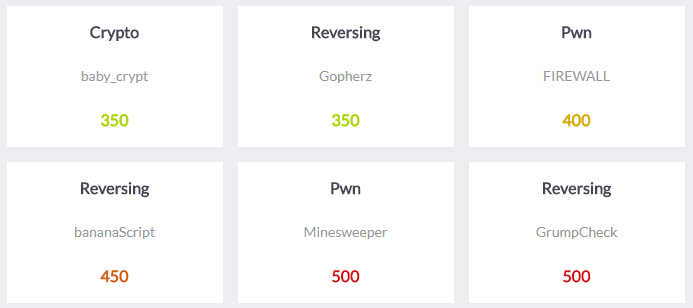
\includegraphics[width=\textwidth]{scoreboard}
    \end{columns}
\end{frame}

\begin{frame}{What's a security capture the flag?}
    \begin{itemize}
        \item<1-> 48 hours of caffeinated reverse engineering and exploitation
        \item<2-> More seriously: an event where you break a bunch of programs
                  to retrieve hidden strings of text (the flags)
        \item<3-> An opportunity to learn new things - we wouldn't
                  even be presenting if it wasn't for this CTF
    \end{itemize}
\end{frame}

\begin{frame}{Who are \VaporSec?}
    \begin{itemize}
        \item A new \Aesthetic San Diego CTF team
        \item Had 10 participants during the CSAW CTF
        \item Got 15th in CSAW industry professional bracket, not bad for
              the first time
    \end{itemize}
\end{frame}
